\documentclass[12pt]{article}
\usepackage[english]{babel}
\usepackage[utf8x]{inputenc}
\usepackage[T1]{fontenc}
\usepackage{lab}
\usepackage{listings}
\usepackage{comment}


\Instructors{Alex Mussa, Kevin Johnson}
\LabNumber{6}
\LabTitle{Sensors and Actuators}
\LabDate{July 12th, 2019}

\lstset{style=mystyle}

\begin{document}
\MakeLabTop

\section{Introduction}

The Arduino nano is a breadboard friendly circuit board whose functionality is centered around the ATMEGA328P microcontroller unit (MCU). This microcontroller contains a processor (CPU) for computational functionality, memory (RAM, ROM), and IO to receive values to be stored in memory and computed with. With these components, the MCU is capable of storing instructions in its memory through a process called programming, and read and execute the program to perform operations on input and output devices, such as LEDs, motors, and various sensors and electronic components. 

The MCU can interact with external devices by reading voltages on its pins (which get digitized either to 1/0, or to a number if using the analog-to-digital converter), processing those values, and outputting other values (always 1/0, but with the capability to produce PWM signals). Since many devices behave differently with different voltages applied to them, this variation can alter some physical phenomena such as motion or light.

In the previous lab, pulse width modulation was used to generate an alternating current signal, as a square wave, that could be used to control LEDs and DC Motors. These types of signals are simple signals to generate for a micrcontroller. In this respect, the microcontroller can be used to read from various sensors, such as the sensor that tells the microcontroller how far the self-balancing robot is tilted. In this situation, if the tilt sensor sends a voltage value to the microcontroller the signifies the robot is tilted forward, then the microcontroller can make the decision to spin the motors by varying the pulse width or duty cycle of the PWM signal in order to catch itself before it falls. 

Microcontrollers have many applications outside of robotics, from children's toys to cellphones. A modern cell phone can contain several microcontrollers, for example. Although several companies make microcontrollers, the one we will utilize and program is an ATMEGA328P, mounted on an open source board developed by the Arduino company. The Arduino NANO board being open-source means that it can be modified and manufactured by 3rd parties. This makes both the hardware and software public domain knowledge and can be re-appropriated without fear of law infringement. This means, for you, that it is less expensive and easier to avoid legal complications if you use them in your design.

The pinout diagram and description of the pins of the Arduino nano can be found below in \textit{Figure 1}.

\begin{figure}[H]
    \centering
    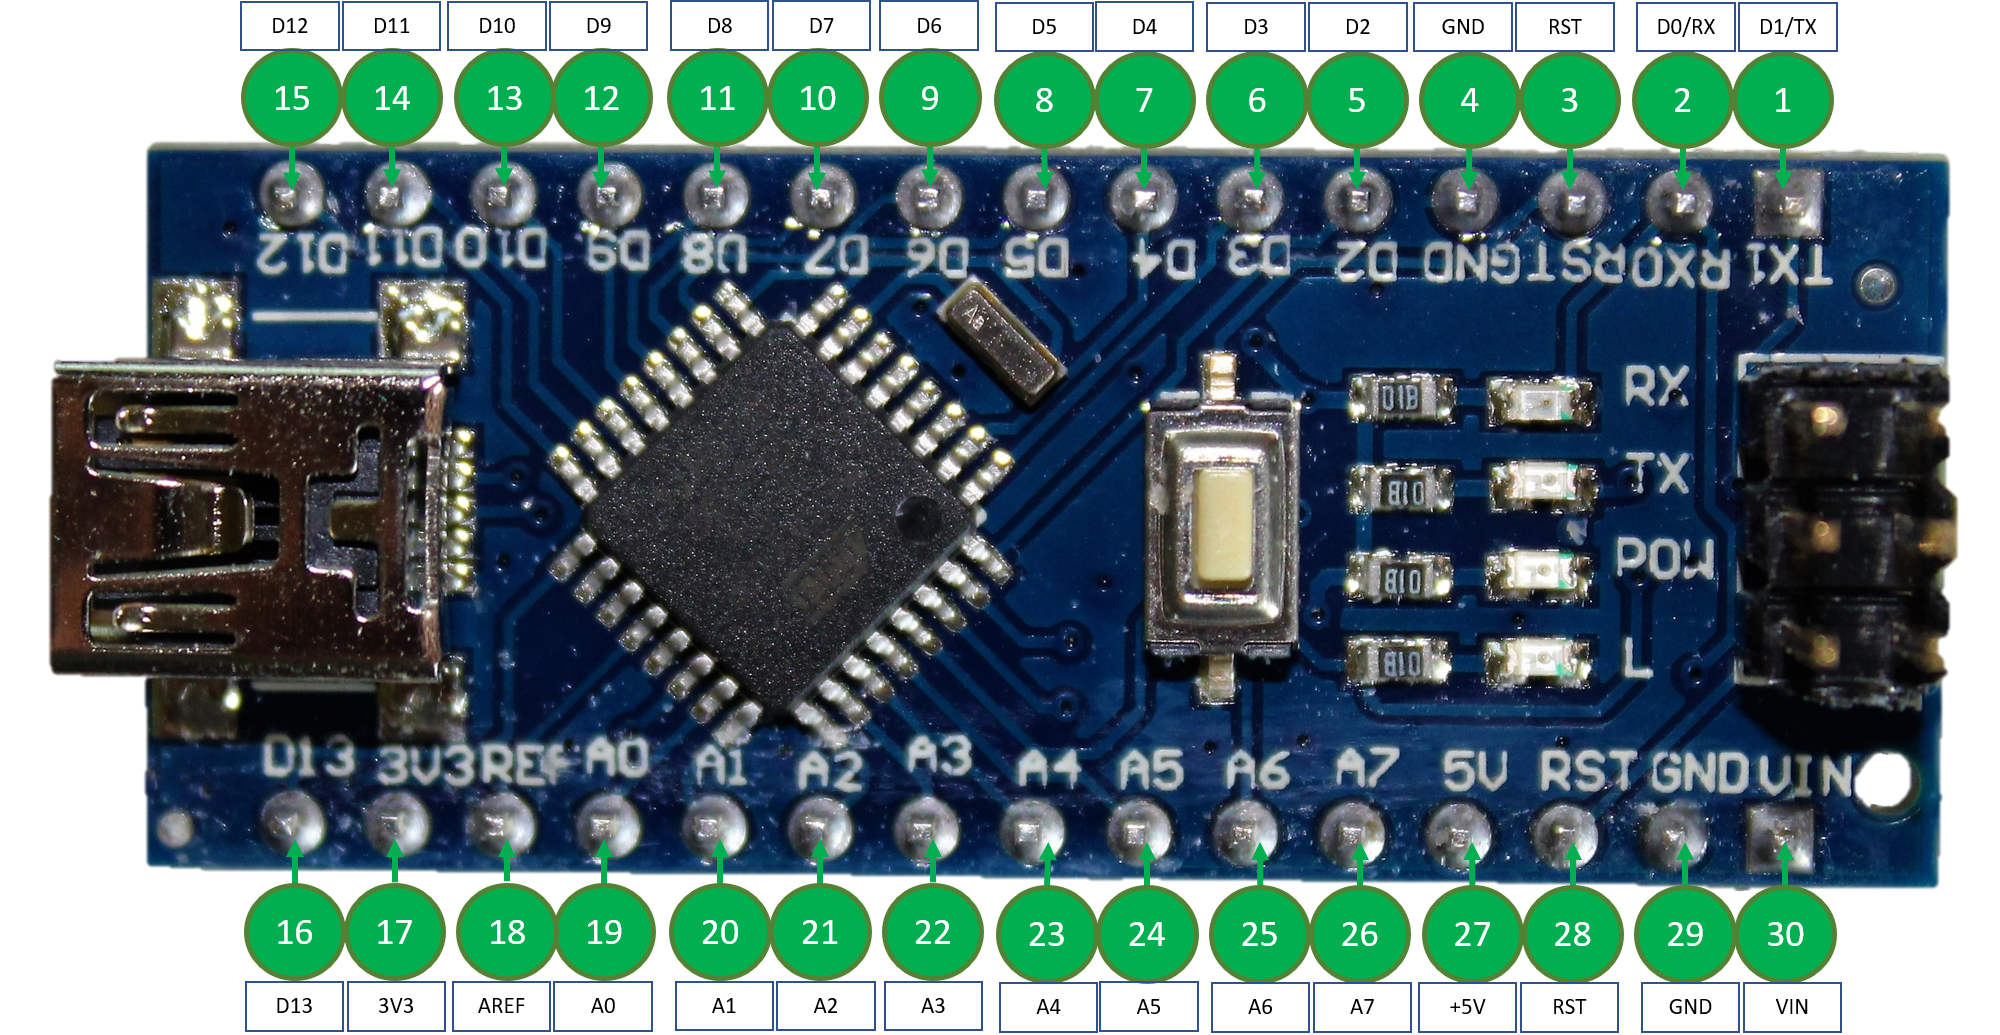
\includegraphics[width=14cm]{photos/lab/nanopinout.png}
    \caption{Pinout for the Arduino Nano V3.0}
\end{figure}

\begin{table}[H]
\centering
\begin{tabular}{|l|l|l|l|}
\hline
Pin No.   & Name   & Type            & Description                                                                                                                \\ \hline \hline
1-2, 5-16 & D0-D13 & I/O             & Digital input/output port 0 to 13                                                                                          \\ \hline
3, 28     & RESET  & Input           & Reset (active low)                                                                                                         \\ \hline
4, 29     & GND    & PWR             & Supply ground                                                                                                              \\ \hline
17        & 3V3    & Output          & +3.3V output (from FTDI)                                                                                                   \\ \hline
18        & AREF   & Input           & ADC reference                                                                                                              \\ \hline
19-26     & A0-A7  & Input           & Analog input channel 0 to 7                                                                                                \\ \hline
27        & +5V    & Output or Input & \begin{tabular}[c]{@{}l@{}}+5V output (from on-board regulator) or +5V \\(input from external power supply)\end{tabular} \\ \hline
30        & VIN    & PWR             & Supply voltage                                                                                                             \\ \hline
\end{tabular}
\caption{Table explaining Arduino Nano's Pinout}
\end{table}

In these lab experiments, we will repeat the experiment of lab 3 that utilized the TB6612FNG motor controller with the signals generated from the lab equipment, but this time the signals will come from the microcontroller. The robot we will use in the final project utilizes these components, and connects them together with a printed circuit board (pcb). In lab 3, we utilized a breadboard to connect them together. In this lab, we will instead utilize the board that connects the components of the robot together, including the Arduino nano, motors, motor controller, and batteries.  You will program the Arduino to input a joystick into the available analog pin on the PCB and use it to control both the direction and speed that a dc motor spins. You will then replace the joystick with a tilt switch to determine direction and a light sensor to vary the speed of the motors.

\section{Setup}

\subsection{Collecting required equipment}

\textbf{\underline{INSTRUCTIONS}}

Collect the following items:
    \begin{enumerate}
        \item Tumbller robot's PCB
        \item If the PCB does not already have an Arduino and/or TB6612FNG Motor Controller installed on it, collect them
        \item Wires (female-to-female recommended)
        \item DC Motor
        \item Motor cable
        \item Batteries and holder (and charger if needed)
        \item 37 Sensor kit
    \end{enumerate}
 \subsection{Connecting to the PCB}
The experiment will require you to build the following circuit with the printed circuit board from the robot:

\begin{figure}[H]
    \centering
    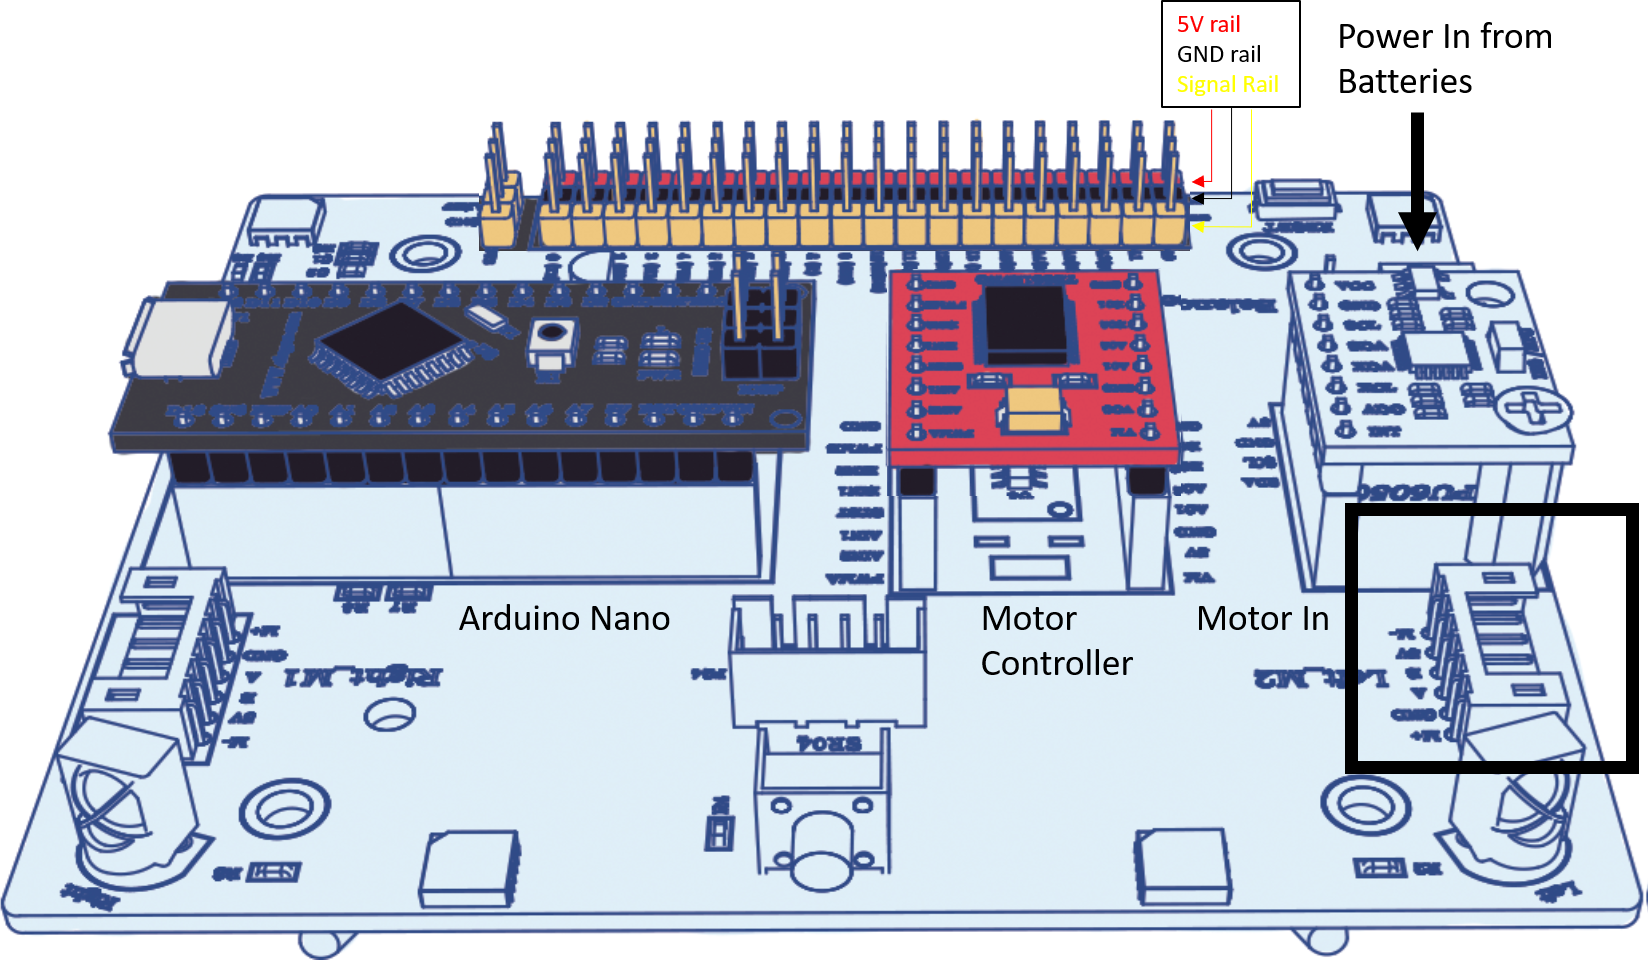
\includegraphics[width=14cm]{photos/lab/pcb.png}
    \caption{Circuit for the Lab 4 experiments.}
\end{figure}

Make sure the motor controller, Arduino nano, battery case, and DC motor are connected to the PCB in their designated locations in \textit{Figure 2}. Note the location of the Signal Rail in yellow at the top of the PCB. This signal rail shows all of the connections used on the Arduino nano, and allows a place to interface with these pins. However, note that many of the pins are physically connected to other components on the circuit board, such as the motor controller, the LEDs, the serial port, etc. There is a general description of what the pin goes to on the PCB next to the signal rail, but a full description can be seen in the below \textit{Table 2}.
\begin{table}[H]
\centering
\begin{tabular}{|l|l|l|}
\hline 
Variable Name          & Pin Number & Description                                                                    \\ \hline\hline
                       & A0         & Free                                                                        \\ \hline
                       & A1         & Free                                                                        \\ \hline
VOL\_MEASURE\_PIN      & A2         & Battery voltage monitoring                                                     \\ \hline
ECHO\_PIN              & A3         & Ultrasonic echo return                                                         \\ \hline
                       & A4 and A5  & I2C pins for the accelerometer/gyro                                            \\\hline
                       & 0 and 1    & Pins for UART.                                                              \\ \hline
ENCODER\_LEFT\_A\_PIN  & 2          & Motor encoder feedback left                                                    \\ \hline
RGB\_PIN               & 3          & LED control                                                                    \\ \hline
ENCODER\_RIGHT\_A\_PIN & 4          & Motor encoder feedback right                                                   \\ \hline
PWMA\_LEFT             & 5          & Motor driver PWM left                                                          \\ \hline
PWMB\_RIGHT            & 6          & Motor driver PWM right                                                         \\ \hline
AIN1                   & 7          & \begin{tabular}[c]{@{}l@{}}motor driver direction left\\   wheel\end{tabular}  \\ \hline
STBY                   & 8          & motor driver enable/disable                                                    \\ \hline
                       & 9          & Free                                                                        \\ \hline
FRONT\_BTN             & 10         & Front pushbutton                                                               \\ \hline
TRIG\_PIN              & 11         & Ultrasonic ping control                                                        \\ \hline
BIN1                   & 12         & \begin{tabular}[c]{@{}l@{}}Motor driver direction right\\   wheel\end{tabular} \\ \hline
                       & 13         & Free                                                                        \\ 
                       \hline
\end{tabular}
\caption{Explanation of signal header pins and where they are connected on the pcb.}
\end{table}

Pins 9, 13, A0, and A1 remain available for interfacing. As such, for this lab, we will only utilize the A0 and A1 pins for programming. 

\subsection{Preliminary Function Reading}

Before beginning with the experiment, please search on the Internet for information on the following functions in Arduino IDE. They will be helpful in the completion of the writing of the code.

\begin{enumerate}
    \item pinMode()
    \item delay()
    \item analogRead()
    \item digitalRead()
    \item digitalWrite()
    \item Serial.begin()
    \item Serial.println()
    \item abs()
\end{enumerate}

Read the Arduino documentation page for each of the functions (search for them using your internet search engine of choice). When you've read through them, continue to the experiment.

\section{Experiments}
\subsection{Joystick Motor Control}

In order to have the hardware in the circuit schematic in \textit{Figure 2} work together as desired, the Arduino will need to be programmed to interface with it. A skeleton code was made for you to start from in order to program the microcontroller to input the joystick and control the motor's direction and speed based on it. To start, download this skeleton code, \texttt{motorcontrol\_skeleton.ino} from canvas and open it. Add your name to the top of the file and read through the comments. Note that the file contains the general structure of an Arduino program file, with variable declarations at the top, the setup() function in the middle, and the loop() function at the bottom. 

\textbf{\underline{INSTRUCTIONS}}
\begin{itemize}
    \item Connect everything to the PCB, including the joystick. The joystick's power and ground will come from the power and ground rails. The Vry signal of the joystick will be connected to the A0 pin at the far right of the Signal Rail. We will not use the Vrx signal in this experiment.
    \item Follow through the skeleton code \texttt{motorcontrol\_skeleton.ino}, downloaded from canvas, from the top to the bottom reading the comments carefully. Add code in the places code is needed as dictated by the comments.
    \item Remember to use print statements and read the terminal for debugging purposes. For example, you can check variable values this way.
    \item To find a function that calculates the appropriate duty cycle for the PWM signal from the joysticks position, it is important to know the value the Arduino sees at the full left, center, and full right positions. To find this, use the print statement provided in the loop function of the skeleton code and open the serial monitor. Adjust the joystick to the positions and record the value in \textit{Table 3}. This will be useful for your code.
    \item When you have completed the code, ensure that the motor operates such that moving the joystick left causes the motor to spin counter-clockwise and moving it right turns the motor clockwise. The center position should have the motor stop, and the amount the joystick is in one direction should determine the speed to which the motor spins. When the joystick is fully right it should go max speed in the clockwise direction, for example.
    \item When you have successfully uploaded the code to the Arduino and the circuit behaves as expected, call the instructor over for a demonstration and proceed to answer the questions below.
\end{itemize}

\begin{table}[H]
    \centering
    \begin{tabular}{|c|c|c|c|} %c means centered left left alighned. Add more | for more lines between columns and more letters for more columns.
        \hline
         &Fully left &  Center & Fully right \\ \hline \hline
         Value&    &     &          \\ \hline %add more of these line for more rows.
    \end{tabular}
    \caption{}
\end{table}

\textbf{\underline{QUESTIONS}}
\begin{enumerate}
    \item Explain the method you used to compute the duty cycle from the joystick input. How were the values in the table used? Why does it achieve what you want it to? 
        \fillwithlines{1in}
        
    \item Why was the battery pack used in the circuit? What does it power and why?  What happens if you turn off the battery pack and run the motor, and what happens if you turn on the battery pack but disconnect the USB cable?
        \fillwithlines{0.7in}

    \item Although the other direction of the joystick was not utilized, what could it have been used for? If you had two motors, what sort of functionality could you add by having the additional direction to the joystick?
        \fillwithlines{1in}

    \item Use your duty cycle function to compute the value of the duty cycle when the joystick outputs a value of 870. State the direction of turn and compute the amount of time the PWM wave is high in milliseconds.
    
        \framebox(439,200){}
\end{enumerate}         

\checkoffsubsub %create a checkoff sub sub section. Details in style file.

\subsection{Tilt switch for direction control and photoresistor for speed control}

In this experiment, you will preform a similar task as the previous, where the Arduino will be programmed to input sensors and use them to control the direction and speed of the motor. However, we will utilize a tilt switch to control the direction and a photoresistor to determine the speed. The tilt switch in the sensor kit outputs high voltage (5V) when upright, and 0V when tilted. A photoresistor is a device that changes its resistance based on light, and the board in the sensor kit has additional circuitry to output a range of voltages depending on the amount of light shining on the device. When more light is shining, the sensor outputs a lower level voltage and when it is covered from the light, a higher level. 

\textbf{\underline{INSTRUCTIONS}}
\begin{enumerate}
    \item Download the skeleton code, \texttt{motorcontrol\_photo\_skeleton.ino} from Canvas and open the sketchbook.
    \item Follow through the sketch and read the comments carefully. Add code where necessary. Program the Arduino to input the tilt switch and photo resistor and control the motor's direction and speed accordingly. 
    \item When you have finished the code, upload it to the Arduino and test the functionality. Hold the tilt switch in one hand and the photoresistor in the other. Make sure the tilt switch changes the direction by tilting the switch and the photo resistor changes the speed by covering and uncovering the sensor with your finger.
    \item When the code works as expected, call the instructor over for verification.
    \item Make sure to save the code with your name in the file name and have two separate files, one for the first experiment and one for the second.
    \item Continue to answer the questions below.
\end{enumerate}

\textbf{\underline{QUESTIONS}}
\begin{enumerate}
    \item How could the tilt be useful for determining the desired direction of the motors in a self balancing robot? Explain your answer.
        \fillwithlines{1in}
        
    \item The photoresistor and tilt switch are just two of many sensors in the sensor kit. Another is a rotary quadrature encoder (rotational position sensor).  Explain one way that the encoder would be used instead of the light sensor.
        \fillwithlines{1in}
        
    \item Another sensor that is common to use is a sonar sensor. This sensor sends out a sound wave and receives it back and computes the two-way travel time, which allows the robot to know how far an object is away up to a certain distance. If a mobile robot was equipped with a sonar sensor, how could that sensor be used to affect the robot's behavior?
        \fillwithlines{1in}
\newpage
    \item What other sensors that you've used or heard of in lecture or your life could be useful for a robot to use in its motor control and why? This could be anything from a camera to a microphone or any other common sensor.
        \fillwithlines{1in}
        
    \item Explain why the threshold the skeleton code used to compute the duty cycle added and subtracted 50 to the room- and covered-brightness values. You can use a plot or words to describe what is happening to the function that computes the duty cycle.
    
        \framebox(439,200){}
        
\end{enumerate}

\checkoffsubsub 

\section{Submission}

When you have finished all of the experiments in \textit{Section 3}, and have received a check off signature with all of the questions answered, you are free to leave. Complete the questions in the packet and bring the packet for submission in the following lab session. Submit the required codes on canvas as well before the next lab session.

\end{document}